%%%%%%%%%%%%%%%%%%%%%%%%%%%%%%%%%%%%%%%%%%%%%%%%%%%%%%%%%%%%%%%%%%%%%%%%%%%%
%  第17回 練習問題［24］〜［30］（旧 prob_p43.png / prob_p44.png / prob_p45.png）
%  ※ このファイルは記録用。実体は physics_ch17.tex に流し込み済み。
%%%%%%%%%%%%%%%%%%%%%%%%%%%%%%%%%%%%%%%%%%%%%%%%%%%%%%%%%%%%%%%%%%%%%%%%%%%%

% 第16回の［23］に続く．章単体で組んだときも番号が本体と一致するように明示しておく
\setcounter{qno}{23}

\filbreak
\Rank{A問題}

\Mon{基本事項の確認}

\hspace{1zw}以下の設問に答えよ．

\hspace{1zw}単原子分子理想気体，二原子分子理想気体の定積モル比熱はそれぞれ$\dfrac{3}{2}R$, $\dfrac{5}{2}R$である．このときそれぞれの比熱比はいくらか．

\filbreak
\Rank{B問題}

\Mon{状態変化に伴う各物理量の変化}

\hspace{1zw}ピストンのついた容器の中に一定量の気体を入れ，次の各変化を行う場合，\MARU{1}\MARU{2}\MARU{3}\MARU{4}に適するものを選べ．
\begin{komon}
\ko{1} 圧力を一定に保って圧縮させるとき
\ko{2} 体積を一定に保って減圧するとき
\ko{3} 温度を一定に保って加圧するとき
\ko{4} 外界との熱のやり取りを断ち切って圧縮するとき
\end{komon}
\hspace{1zw}各状態変化において，
\begin{list}{}{\setlength{\leftmargin}{2zw}\setlength{\itemsep}{0.4mm}\setlength{\topsep}{0.6mm}\setlength{\parsep}{0pt}}
\item[・] 外界が気体に与える熱量$Q$は，\fbox{\MARU{1}：正，\,0，\,負}となる．
\item[・] 外界が気体に対してする仕事$W$は，\fbox{\MARU{2}：正，\,0，\,負}となる．
\item[・] 気体の内部エネルギーの変化量$\Delta U$は，\fbox{\MARU{3}：正，\,0，\,負}となる．
\item[・] 気体の温度は，\fbox{\MARU{4}：上昇する，一定である，下降する}．
\end{list}

\Mon{定温変化}

\begin{zuright}{58mm}
\hspace{1zw}右図のように断面積$S\U{m^2}$のシリンダーの中に，ピストンで定積モル比熱が$C_V\U{J/mol\cdot K}$の理想気体を$n\U{mol}$だけ封入した．ピストンは軽くて自由に動くことができ，棒が取り付けられてある．
\zusep
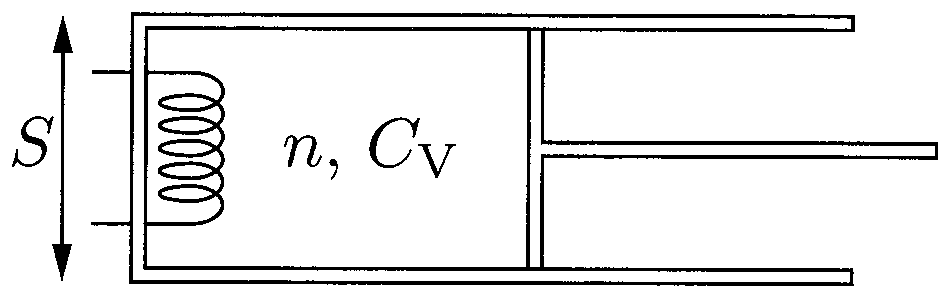
\includegraphics[keepaspectratio,width=58mm]{fig/ch17_p43_cyl.png}
\end{zuright}
\hspace{1zw}初め，シリンダーの底からピストンまでの距離は$l_0\U{m}$であり，また気体の温度は$T_0\U{K}$であった．シリンダー内にはヒーターが取り付けられており，気体に対して熱を与えることができる．シリンダーおよびピストンは断熱材でできており，ヒーターによって与えた熱が大気に拡散することはないものとする．気体定数を$R\U{J/mol\cdot K}$として以下の設問に答えよ．
\begin{komon}
\ko{1} 初めの状態におけるシリンダー内の気体の圧力$p_0\U{Pa}$を求めよ．
\end{komon}
\hspace{1zw}ここで，気体が温度$T_0\U{K}$を保つようにピストンを操作しながら内部の気体をヒーターでゆっくりと加熱したところ，ピストンはゆっくりと移動し，シリンダーの底からピストンまでの距離が$l_1\U{m}$となったところで加熱をやめた．
\begin{komon}
\ko{2} 終状態における気体の圧力$p_1\U{Pa}$を求めよ．
\ko{3} この変化において，気体が外界にした仕事$w\U{J}$を求めよ．
\ko{4} ヒーターによって加えた熱量$Q\U{J}$を求めよ．
\end{komon}

\Mon[\Sitei]{断熱変化}

\begin{zuright}{58mm}
\hspace{1zw}右図のように断面積$S\U{m^2}$のシリンダーの中に，ピストンで定積モル比熱が$C_V\U{J/mol\cdot K}$の理想気体を$n\U{mol}$だけ封入した．ピストンは軽くて自由に動くことができ，棒が取り付けられてある．
\zusep
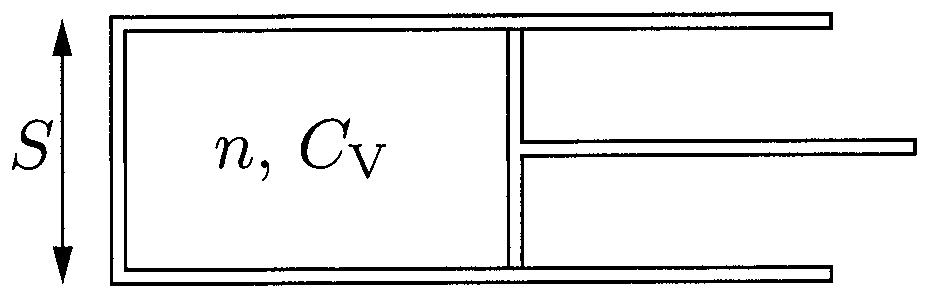
\includegraphics[keepaspectratio,width=58mm]{fig/ch17_p44_cyl.png}
\end{zuright}
\hspace{1zw}シリンダーおよびピストンは断熱材でできており，外界と熱のやり取りはない．棒を手で持って動かし，シリンダーの底からピストンまでの距離が$l_0\U{m}$となる位置に持ってきたところ気体の温度は$T_0\U{K}$となった．気体定数を$R\U{J/mol\cdot K}$として以下の設問に答えよ．
\begin{komon}
\ko{1} この状態におけるシリンダー内の圧力$p_0\U{Pa}$を求めよ．
\end{komon}
\hspace{1zw}ここでピストンを手でゆっくりと引き，シリンダーの底からピストンまでの距離が$l_1\U{m}$になるまで気体を膨張させた．
\begin{komon}
\ko{2} ポアソンの法則を用いて，終状態における気体の圧力$p_1\U{Pa}$および温度$T_1\U{K}$を求めよ．
% 誤植訂正（2026-09-02）：原本は「温度 T_1[K] 求めよ」で助詞「を」が欠けていた．
\ko{3} この状態変化を$p-V$図で表せ．
\ko{4} この変化において，気体が外界にした仕事$w\U{J}$を求めよ．
\end{komon}

\Mon{断熱自由膨張}

\begin{zuright}{56mm}
\hspace{1zw}右図のように，体積$V_\mathrm{A}\U{m^3}$, $V_\mathrm{B}\U{m^3}$の断熱容器A，Bをコックのついた細い管でつないである．はじめコックは閉じられており，Aだけに定積モル比熱$C_V\U{J/mol\cdot K}$の理想気体が圧力$p_0\U{Pa}$，温度$T_0\U{K}$となって入っている．コックを開いたところ気体はBへと拡散していき，十分時間が経つと全体が一様となった．このときA，B内の気体の圧力および温度を求めよ．ただし，気体定数を$R\U{J/mol\cdot K}$とする．
\zusep
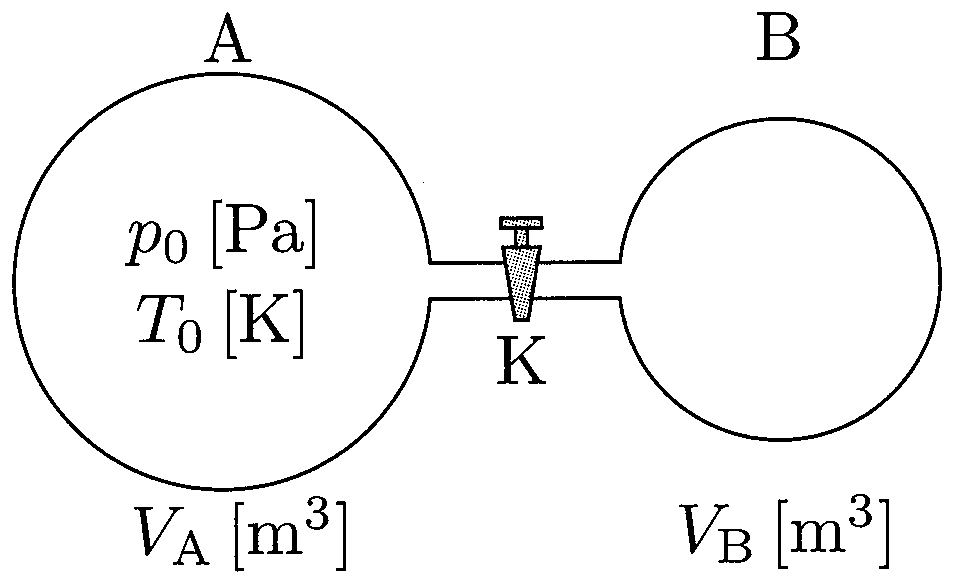
\includegraphics[keepaspectratio,width=56mm]{fig/ch17_p44_ab.png}
\end{zuright}

\Mon[\Sitei]{断熱膨張・断熱自由膨張}

\begin{zuright}{56mm}
\hspace{1zw}右図のようにバルブつきの隔壁で仕切られたシリンダーがある．隔壁の左側の体積は$V_0\U{m^3}$であり，ここに定積モル比熱$C_V\U{J/mol\cdot K}$の理想気体が圧力$p_0\U{Pa}$，温度$T_0\U{K}$となって封入されている．
\zusep
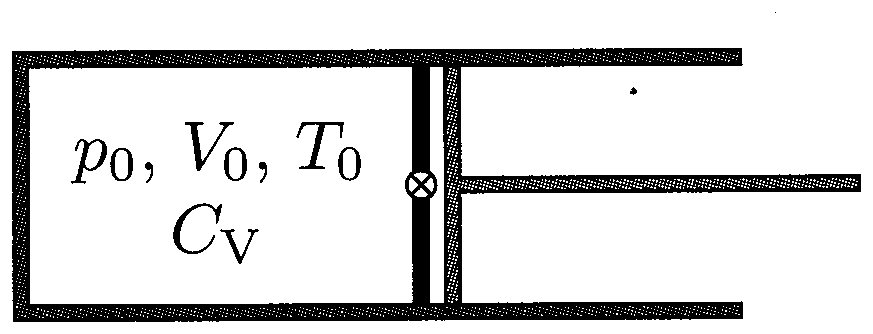
\includegraphics[keepaspectratio,width=56mm]{fig/ch17_p44_valve.png}
\end{zuright}
\hspace{1zw}隔壁の右側は取っ手付きのピストンが取り付けられている．初めバルブは閉じており，右側の空間には気体は封入されておらず，ピストンは隔壁に接触して体積が0になっている．シリンダー，ピストン，隔壁，バルブなどはすべて断熱材で出来ており，外界との熱のやり取りはない．

\hspace{1zw}この状態から以下の二つの方法によって左側に封入されている気体を右側に拡散させる．このとき，終状態における気体の圧力および温度をそれぞれ求めよ．気体定数を$R\U{J/mol\cdot K}$とする．
\begin{komon}
\ko{1} バルブを閉じたまま取っ手を引いて右側に体積$V_0\U{m^3}$の真空を作ったのち，バルブを全開にして気体を右側へ拡散させる．
\ko{2} バルブを全開にしてから取っ手をゆっくりと引き，右側の空間の体積を少しずつ増加させて体積$V_0\U{m^3}$にする．
\end{komon}

\filbreak
\Rank{C問題}

\Mon{気体の一般的な状態変化}

\begin{zuright}{62mm}
\hspace{1zw}図のように断面積$S\U{m^2}$のシリンダーに定積モル比熱が$C_V\U{J/mol\cdot K}$の理想気体を封入し，ピストンに図のように弾性定数が$k\U{N/m}$のバネを取り付けた．バネが自然長のとき，ちょうど大気圧$P_0\U{Pa}$とシリンダー内の気体の圧力とがつり合い，このときの気体の温度は$T_0\U{K}$，気柱の長さは$l_0\U{m}$であった．
\zusep
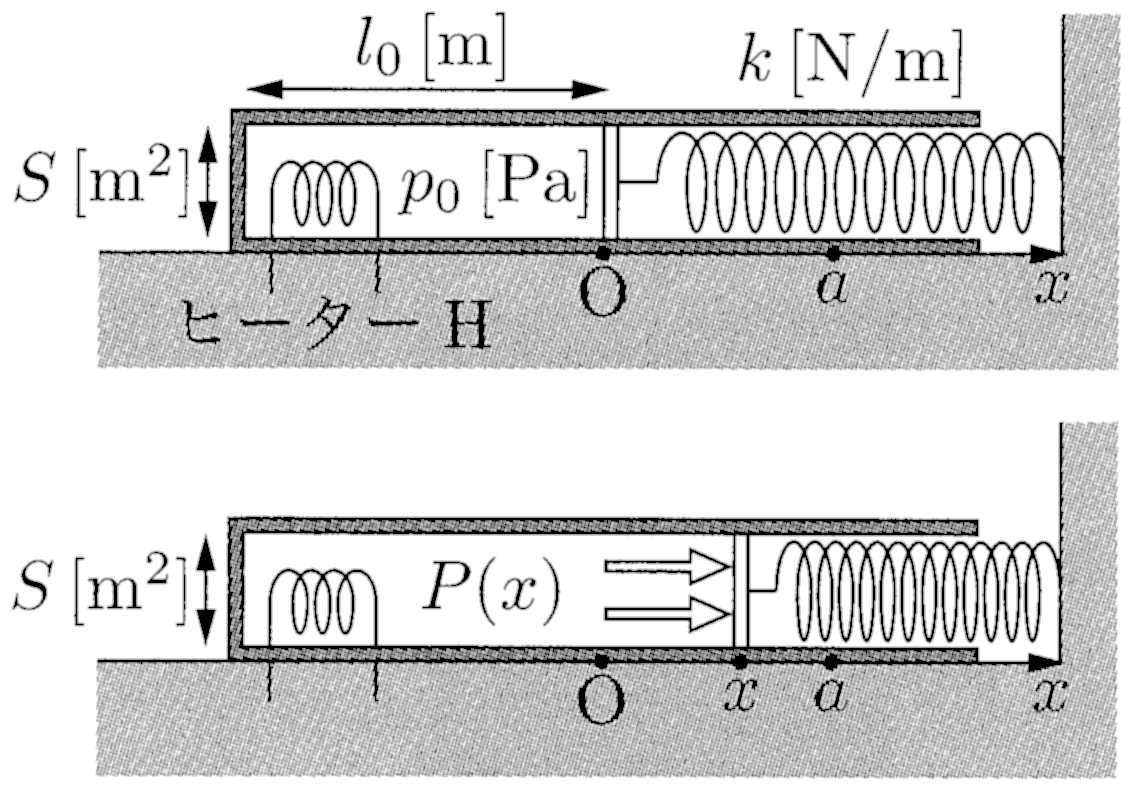
\includegraphics[keepaspectratio,width=62mm]{fig/ch17_p45_spring.png}
\end{zuright}
\hspace{1zw}シリンダー内のヒーターHから少しずつ気体を加熱していったところ，気体はゆっくりと膨張し，ピストンはゆっくりと距離$a\U{m}$だけ進んだ．シリンダー，容器などはすべて断熱材で出来ており，バネなどの熱容量は無視してよい．気体定数を$R\U{J/mol\cdot K}$として以下の設問に答えよ．
\begin{komon}
\ko{1} 終状態における気体の圧力$P_1\U{Pa}$および温度$T_1\U{K}$を求めよ．
\ko{2} この状態変化で気体がする仕事$w\U{J}$を求めよ．
\ko{3} この状態変化で気体に与えた熱量$Q\U{J}$を求めよ．
\end{komon}
